\documentclass{article}
\usepackage{fullpage}
\usepackage{amsmath,amssymb}
\usepackage{natbib}
\usepackage{marginnote}
\usepackage{graphicx}
\usepackage{hyperref}
\usepackage{latexml} % for \iflatexml
\usepackage{color}
\newcommand{\gc}[1]{{\it\color{green}(#1)} }
\newcommand{\plr}[1]{{\it\color{blue}(#1)}}

\newcommand{\var}{\mathop{\mbox{Var}}}
\renewcommand{\P}{\mathbb{P}}
\newcommand{\E}{\mathbb{E}}
\newcommand{\R}{\mathbb{R}}

\iflatexml  % no margin notes in latexml
% \newcommand{\marginnote}[1]{}
\newcommand{\marginnote}[1]{{\it\color{red}(#1)}}
\fi

\bibliographystyle{plain}

\begin{document}

\section{Introduction}



In \citep{RalphCoop} we formulated a simple model of parallel adaptation in a geographic setting
where the selection pressure was constant across the entire environment, 
and that a single mutational change was sufficient to adapt populations to the novel environment. 
We assumed that there was no standing variation for the adaptive allele, such that parallel mutation must be due to multiple mutations after the environmental shift. In that setting we found that there was a characteristic geographic scale, over which we would expect multiple instances of our adaptive allele to have arisen in parallel. This characteristic length could be expressed in terms of a simple compound parameter determined by our parameters of interest.
Recall questions of origin of adaptations

References on parallel adapation, standing variation, etc.:
  coop,
  pennings and hermisson.
Note pennings and hermisson found standing deleterious variation was very important.  

recall peromyscus examples with patchy environments

Summarize previous paper

Question assumptions of no standing variation and homogenous selection

\section{General model}

outline here assumptions common to both models.

Stick to constant-speed waves.
Note monty's empircal speeds paper.


\section{Standing variation}

\subsection{The set-up}

% selection pressure changes at $t=0$ from $1-s_d$ to $1+s_b$ -- homogeneous

We assume that the species range
is a homogenous, one- or two-dimensional region. 
There are two selective classes -- the {\em neutral} type, and the {\em mutated} type.
We assume that different mutations are distinguishable --
either as selectively equivalent mutations, or by linked variation.
For a long time in the past, the mutated type has been at a selective disadvantage (long enough to be at selection-mutation equilibrium),
but at a certain time the selective regime changes, so that the mutated type has a selective advantage and quickly spreads to fixation.
After fixation, alleles are either descended
from families of mutants present as standing variation when the selective regime changed,
or from new mutants arising since that time.

For concreteness, suppose that before time $t=0$,
the mutant type has fitness $1-s_d$ relative to the neutral type
(i.e.\ it produces on average $1-s_d$ times the number of offspring per generation),
and that after time $t=0$,
the mutant type has fitness $1+s_b$,
where $s_b>0$ will usually be assumed to be small, and $0<s_d<1$.
We assume that diploid fitness is additive, or at least that the
important early dynamics are determined by the haploid fitness
\gc{heterozygous fintess, with no reference to the fitness of the
  homozygote for the mutant alleles}.
The number of offspring has finite variance, which to keep the formulas simple we assume to be equal to one.
(If the mutation is recessive, XXX more complicated things happen.)
As for the other parameters,
suppose that each offspring of a neutral parent is of the mutant type with probability $\mu$,
and that the mean squared distance between parent and child is $\sigma^2$ (the {\em dispersal variance}).
The species occupies an area with mean density
$\rho$ haploid individuals (or chromosomes) per unit area.
\marginnote{XXX or do diploid? below is haploid.}


% Branching-process-sized point mass approx to local groups present at $t=0$
% -- depends on local population density large enough relative to migration (to be "branching")
% -- and migration not too large (since we approximate as a point mass).
% Find mean density of clusters of successful standing mutants. 
% Is greater-than-one size of clusters likely to make a difference? 

\paragraph{Rates of origination of standing and new mutations}
We make use of the commonly used approximation that neglects competition between relatives,
treating the offspring of a new mutant that appears in an area not already occupied by the mutated type
as a branching process.
After $t=0$, the offspring of a single mutant form (approximately) a branching process with growth rate $s_b$,
so each new mutant establishes locally with probability $p_s \approx 2s_b$.
As in \cite{ralphcoop2010}, each new offspring has a very small probability of being a mutant and establishing locally,
so the collections of times and locations at which mutants appear and establish locally 
is well--approximated by a Poisson process in space and time.
This the rate of this Poisson process, 
the rate per unit area at which new mutants appear and establish locally after $t=0$ in areas not already occupied by the mutant type
is approximately $\lambda = 2 \mu \rho s_b$.



Before $t=0$, on the other hand, the mutation is deleterious, so the
genetic descendents of each new mutation are (with high probability)
doomed (doomed I say!) to extinction,
but may persist for some time.
Since the times and locations of mutants before $t=0$ also well-approximated by a Poisson process with rate $\mu \rho$,
the locations of all mutant families extant at $t=0$ whose descendents are destined to fix locally is also,
by the Mapping theorem, a Poisson process with rate we define to be $\lambda_0$.
If we assume that the descendants of at most only a few members of any extant mutant family at $t=0$ will survive,
and that these progenitors are near to each other in space, we can then treat each such family as a single mutant,
equivalent to the mutants arising later.
(The approximation will be good if the log of the size of an extant families is small relative to the establishment time,
and the spatial distribution of the family is small relative to the spread between them.)
To find $\lambda_0$, consider a mutation that arose at time $-T<0$, and let $Z_s$ be the number of its descendants at time $s-T$.
At time $t=0$, there are $Z_T$ individuals present with the mutation,
and each has probability $p_s \approx 2s_b$ of establishing, approximately independently.
Therefore, the probability that some descendants of this mutation establish and fix locally is $1-(1-p_s)^{Z_T}$,
so defining $\zeta(u,t) = \E[u^{Z_t} | Z_0=1 ]$ to be the generating function of $Z_T$,
the rate is
\begin{align*}
    \mu \rho \int_0^\infty \left( 1- \zeta(1-p_s,T) \right) dT .
\end{align*}
Now for $s_b$ small, using $p_s \approx 2s_b$ and that $\E[Z_T]=(1-s_d)^T$,
we know that $\zeta(1-2s_b,T) \approx 1-2s_b \E[Z_T] = 1-2s_b (1-s_d)^T$,
resulting in the approximation
\begin{align}
    \lambda_0 &= \mu \rho \int_0^\infty 2s_b (1-s_d)^{T} dT \\
        &= \frac{ 2 \mu \rho s_b }{ -\log(1-s_d) } .
\end{align}


\plr{XXX More discussion on whether this is a good approximation?  
Compute typical size and radius of a standing cluster?}
\gc{Point out connection to standard mutation selection balance formula}


\paragraph{Geographic spread of alleles} 
Once an allele has become local established it can begin to spatially spread. 
We assume that the allele, having become established, quickly settles
down to spread as a traveling wave of constant speed. The behavior of
this wave of advance of a beneficial allele was first described by 
\citet{fisher1937wave} and \citet*{KPP1937}. 

If the mean squared distance between parent and child is $\sigma^2$
(i.e.\ $\sigma$ is the dispersal distance) then the speed of advance
of this wave will be $v = \sigma \sqrt{2s}$. 

\plr{recall PPP computations; draw cones of opportunity for new mutations }

\paragraph{}
So we can put these ingredients together for a simple model of the
geographic spread of alleles. A cartoon example of this process is
shown in Figure \ref{fig:cartoon} Initially, when the selection
pressures change at $t=0$, a set of standing variants can start to
spread having escaped loss through drift. These variants are shown as
little lightning bolts, and occur at a density $\lambda_0$ across
space. 
They spread at velocity $v$ carving out cones in space-time. As these
alleles proceed in their geographic spread other new alleles can arise
and become established in parallel, these are shown as little
stars. These new mutations arise and become established at rate $\lambda$.

The wave of advance works in the case of heterozygote advantage
\citep{aronson1975nonlinear}, with the selected allele spreading
locally to the equilibrium frequency (rather than fixation). As such
our framework is applicable here.

\begin{figure}[ht]
  \begin{center}
    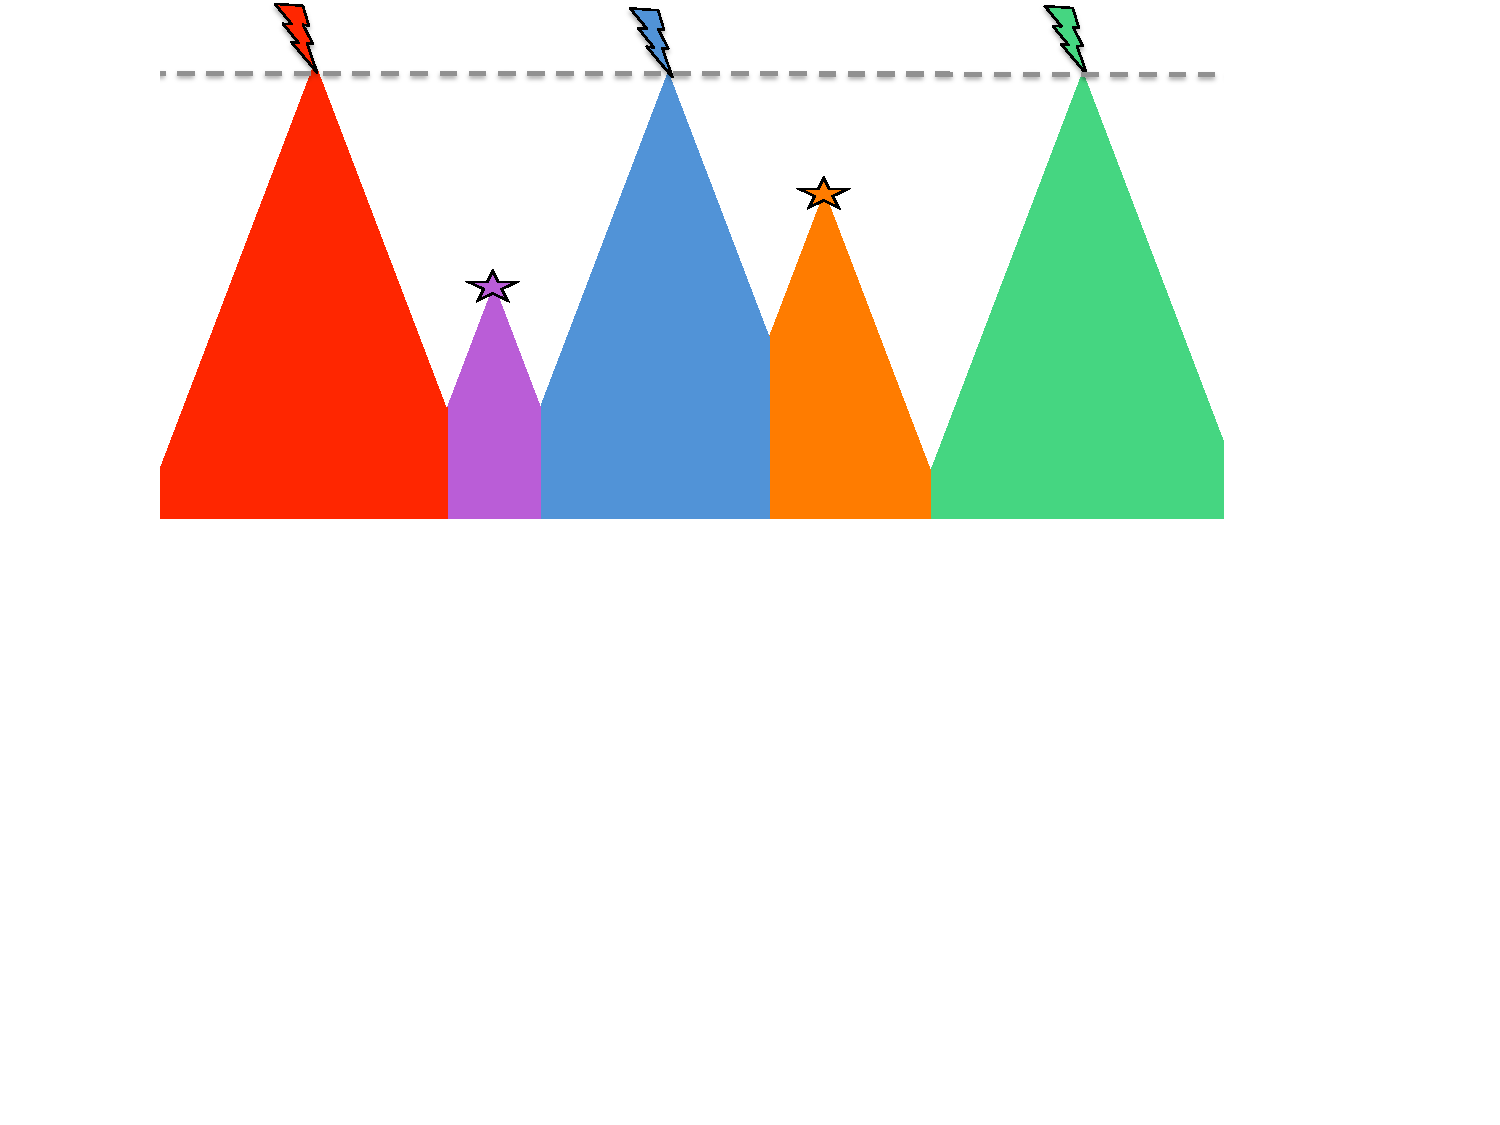
\includegraphics{spreading_alleles_trimmed}
  \end{center}
  \caption{
Cartoon of the geographic spread of standing and new mutations. 
}
  \label{fig:cartoon}
  
\end{figure}



\subsection{G6PD}

Over the past ten thousand years malaria resistance alleles have arisen at a number
of genes and spread through human populations in areas where malaria is endemic \citep{Kwiatkowski:05}. 
A number of these alleles appear to represent convergence, with
multiple changes in the same gene. 
For example, there are multiple
changes at the $\beta$-globin gene that confers malaria resistance,
and the sickle cell allele may plausibly have arisen by up to five distinct
changes at the same base pair within Africa
\citep{Flint:98,ralph2010parallel}.
Another particularly impressive case of convergent evolution in response to
selection pressures imposed by malaria are the numerous changes throughout the
X-linked G6PD gene, with upward of 50 polymorphic variants ($>1\%$ frequency) having so far been
described that lower the activity of the enzyme \citep{Howes-g6pd-variants,Minucci-g6pd}. These alleles are now
found at a combined frequency of $\sim$8 \% frequency in malaria endemic countries, rarely
exceeding$\sim$20 \% \citep{Howes-g6pd-preval}. Three malaria
resistance alleles at G6PD are particularly common and relatively well
studied: the $A-$ found in
much of sub-Sharan Africa; the Med allele found in the Mediterranean and middle
east; and the Mahidol allele found Myanmar and Thailand.
The $A-$ and Mahidol alleles have been shown
to be protective against {\it Plasmodium falciparum} and {\it P. vivax} in both
hemizygote males and both heterozygote and homozygotes females \citep{Ruwende-g6pd ,
Louicharoen-g6pd}. Haplotype-based analysis of genetic diversity surrounding
the $A-$, Med, and Mahidol suggest that they have spread in past few
thousand years \citet{tishkoff-g6pd, Slatkin-age-est,Saunders-g6pd,Louicharoen-g6pd}, 
consistent with the age of other malaria resistance alleles. 
These population genetic analyses suggest that three variants each have a hemizygote/heterozygote 
selection coefficient of $0.05-0.3$ \citep{tishkoff-g6pd
  Slatkin-age-est,Saunders-g6pd,Louicharoen-g6pd}, consistent with
the results of \citet{Ruwende-g6pd} on the basis of the present day increased resistance to malaria of the
$A-$ allele. 
Given such a strong pressure on these alleles they should have risen
quickly to fixation, so their prescence at intermediate frequency,
over a broad geographic area, makes it a good candidate for a recently
balanced polymorphism. 
Hemizygous males and homozygous females suffer from G6PD deficiency,
leading to hemolytic anemia when exposed to various compounds, notably
those present in fava beans. 


% G6PD frequency across world http://www.google.com/imgres?imgurl=http%3A%2F%2Fwww.plosmedicine.org%2Farticle%2Finfo%3Adoi%2F10.1371%2Fjournal.pmed.1001339.g002%2Flargerimage&imgrefurl=http%3A%2F%2Fwww.plosmedicine.org%2Farticle%2Finfo%253Adoi%252F10.1371%252Fjournal.pmed.1001339&h=2938&w=2381&tbnid=oD_tX3ea8IbLfM%3A&zoom=1&docid=k37axqAZDS7ljM&ei=5rdOU5TVDMqj8QGntICYBg&tbm=isch&ved=0CF8QMygLMAs&iact=rc&uact=3&dur=1447&page=1&start=0&ndsp=15

% Spatial distribution of G6PD alleles:  http://www.malariajournal.com/content/12/1/418




%Hedrick sex-specific review http://www.eeslmu.de/eeswiki/images/Hedrick_Review.pdf
% Fry: http://www.ncbi.nlm.nih.gov/pmc/articles/PMC3654548/
% kidwell http://www.ncbi.nlm.nih.gov/pmc/articles/PMC1213615/
%Rice: http://www.jstor.org/discover/10.2307/2408385?uid=3739560&uid=2129&uid=2&uid=70&uid=4&uid=3739256&sid=21103992458511

%IDEA: could we look at all freq. reports of g6pd and see if male and
%female freq. diffs support model of sexual-conflict?

The geographic area of Central and Eastern Asia with malaria is on the
order of $\sim 10$ million $km^2$. In that area there are at least $15$
common variants \citep{Howes-g6pd-variants}. So the average width of
an area occupied by an allele is $\sqrt{10^7/15} \approx  800$km. 


G6pd is 515 codons long, with 140 variants reported in it REF. Assuming a
mutation rate of $\approx 10^{-8}$ per base-pair per generation, we assume
$\mu \approx 1 \times 10^{-6}$ a generation. 
The dispersal and demographic parameters of humans is unclear,
particularly as we are concerned with the effective population density.
We use $\rho=2$ and $0.2$ people per $km^2$ as two choices of our effective population density.
We use $\sigma=10,~50,$ and $100$ as our dispersal parameter.

\begin{figure}[ht]
\begin{center}
  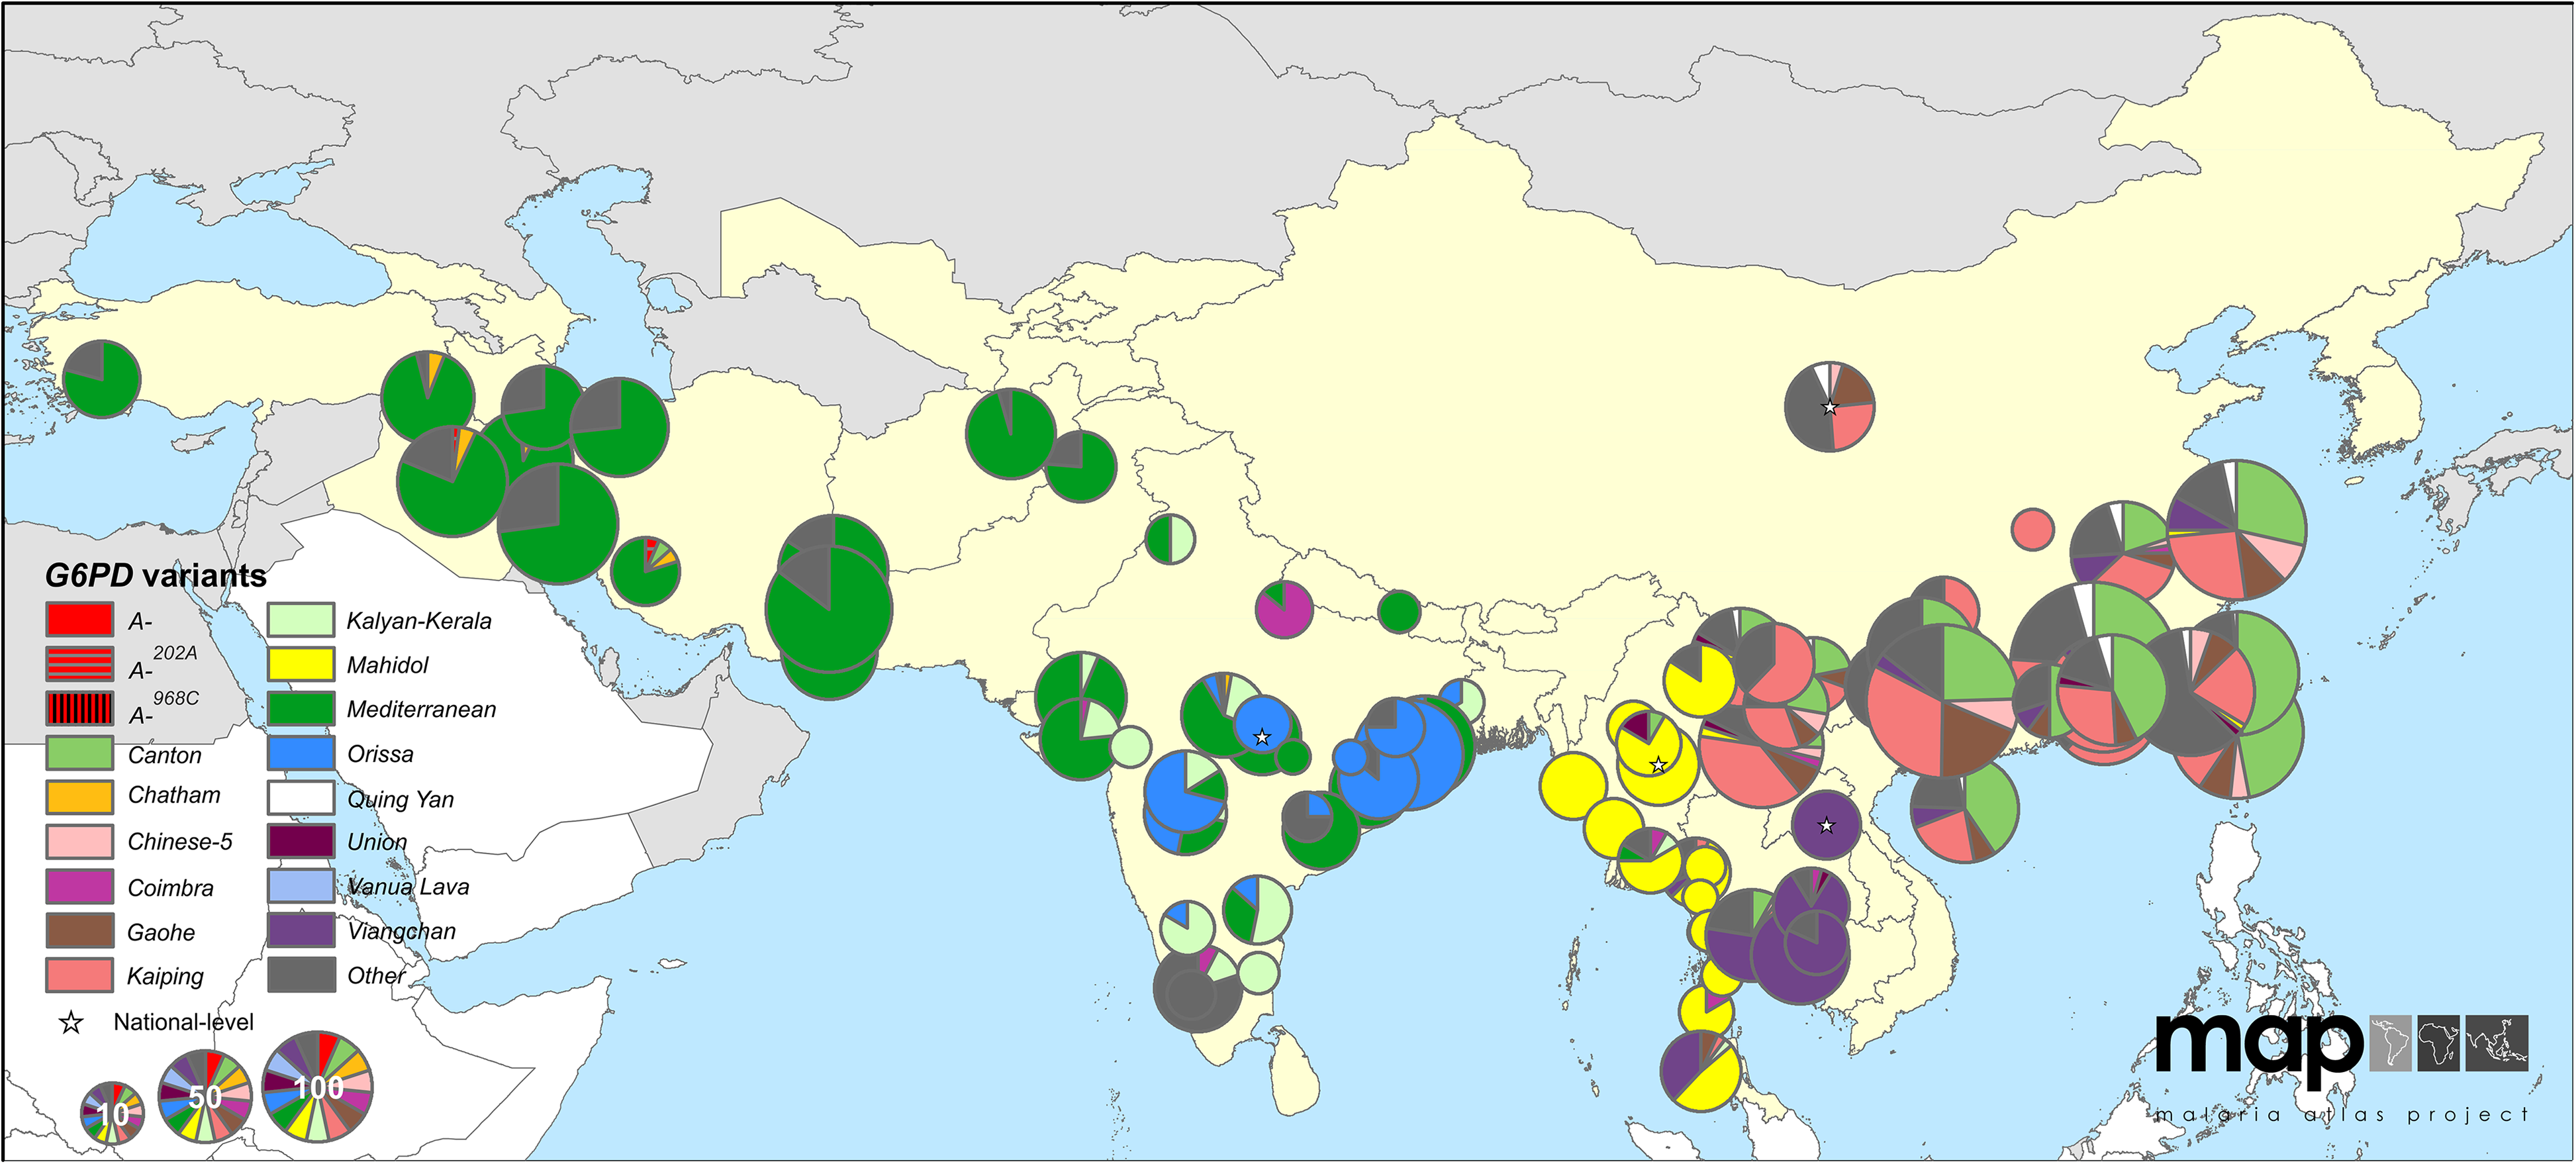
\includegraphics[width=1.0\textwidth]{G6pd_Howes_et_al_1475-2875-12-418-4}   %{charlen-by-sd-limit}
\caption{ %
{\bf Map of G6pd-deficiency allele frequencies across Asia.} The pie chart shows
  the frequency of G6pd-deficiency alleles. Size of the pie chart
  indicates the number of G6pd-deficient individuals sampled.
. Countries with
  endemic malaria are colored yellow. Figure taken from
  \citet{Howes-g6pd-variants} \url{http://www.malariajournal.com/content/12/1/418}.
}
\end{center}
\end{figure}

% \begin{figure}[ht]
% \begin{center}
%   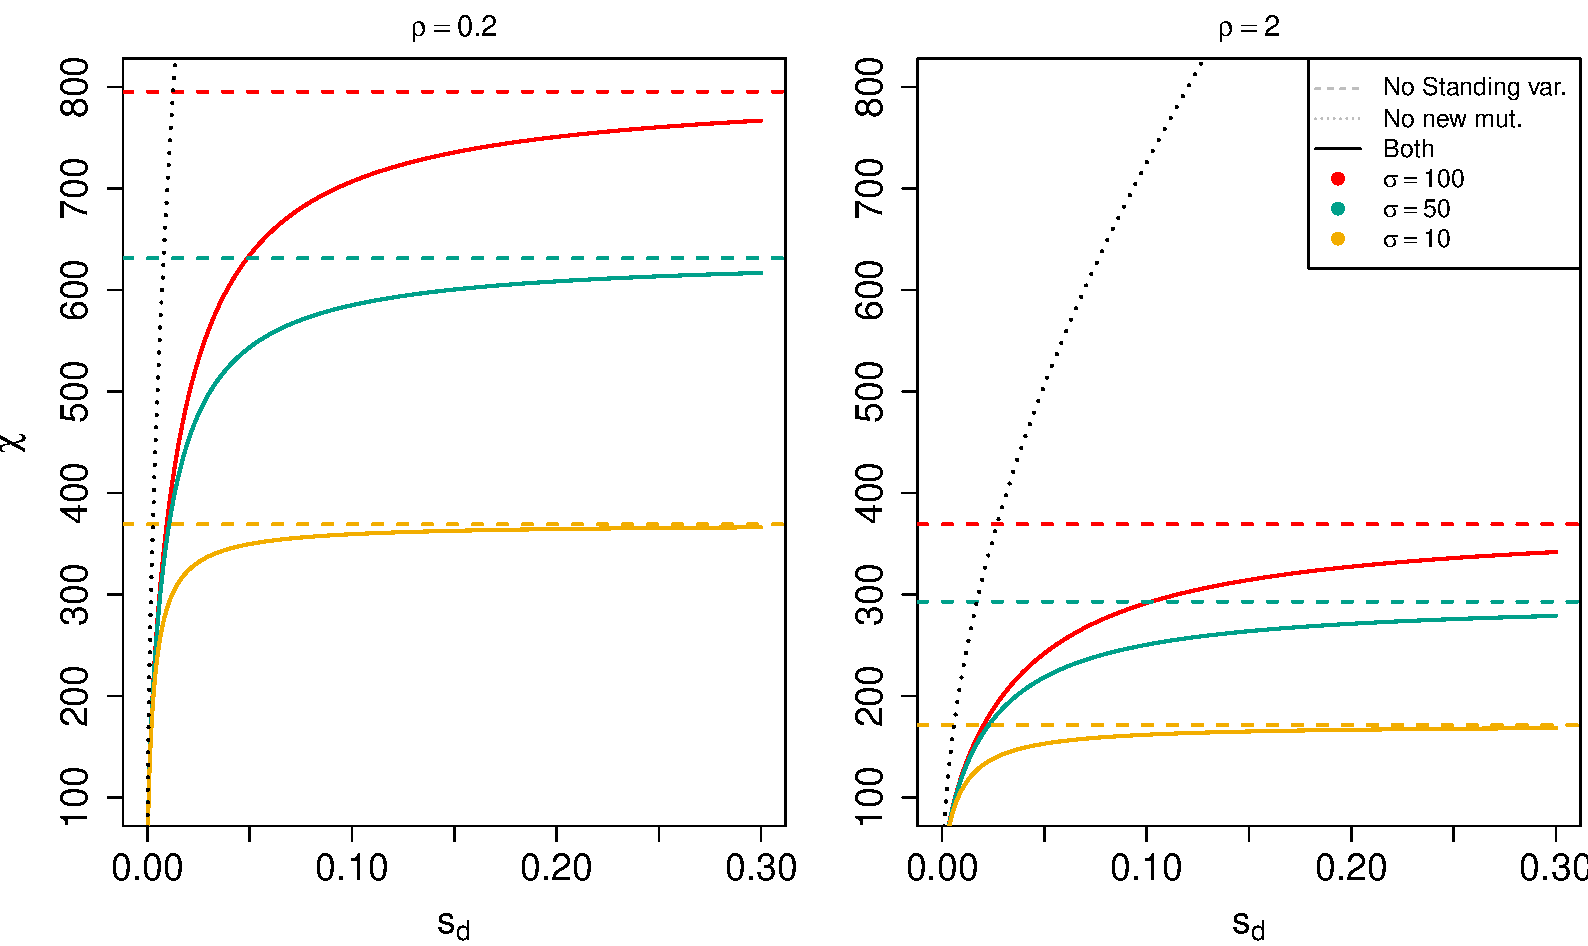
\includegraphics[width=1.0\textwidth]{G6PD_charlengths}
% \caption{ %
% {\bf Characteristic length,} as a function of dispersal distance $\sigma$ and selective disadvantage $s_d$.  XXX at what parameters. XXX
% } \label{Fig-G6PD-charlength}
% \end{center}
% \end{figure}



%$A-$ ?? risk lower of severe malaria for both female heterozygotes and male
 %hemizygotes estimates of selection pressure \citep {Ruwende-g6pd}
%Mahidol487A \citep{Louicharoen-g6pd}
%Show's effect in het and homozy females


%Selection coefficient (s) 	A- 0.044 (0.019–0.048)  Med	0.034
%(0.014–0.049)  ``The mean age of the A− allele in these runs was 6357 years, with a 95\% credibility interval extending from 3840 to 11,760 years. For the Med alleles, the mean age was 3330 years with a 95\% credibility interval of 1600 to 6640 years"
%\citet{tishkoff-g6pd}
%s 0.24 and t= 40 generations \citep{Slatkin-age-est}
%The estimated age is ~100 generations with an upper bound of <150
%generations A- 0.1 < s < 0.2 \citep{Saunders-g6pd}
%Mahidol487A mutation started to increase at ~1500 YBP, with a
%selection intensity of ~0.23 \citep{Louicharoen-g6pd}
%Show's effect in het and homozy females

\subsection{Characteristic parameters}

% a characteristic length of regions and a proportion of haplotypes (or of space?) that are from standing variation

In \citet{ralphcoop2010}, studying the model without standing variation,
we defined a {\em characteristic length} which gave the spatial scale across with mutants with distinct origins would establish.
This was proportional to the mean distance between neighboring established mutants,
but had the advantage of being easier to calculate.
Furthermore, the time scale over which adaptation occurred could be found by dividing the characteristic length 
by the speed at which the mutants spread.
We will define the characteristic length for this new model,
as well as a similar compound parameter describing the relative importance of standing variation to the process of adaptation.
%(Note that a similar approach, summarizing with a {\em characteristic length} was taken by \citep{slatkin1973geneflow} for a different problem.)

Suppose we fix our attention on a particular new mutation that happens to be the first to occur in some region.
As it spreads, it will cover a distance $L$ in time $L/v$.
The number of other mutations appearing in the circle it has covered up until this time is Poisson with mean
$\lambda_0 \pi L^2 + \lambda \pi L^3 /v$ in two dimensions
(and $\lambda_0 2 L + \lambda \pi L^2 /v$ in one dimension).
% $\lambda_0 \omega_d L^d + \lambda \omega_d L^{d+1} /v$ in $d$ dimensions
Therefore, if we define $\chi$ to be the unique positive solution to
\[
    \lambda_0 \pi \chi^2 + \lambda \pi \chi^3 /v = 1,
\]
then $\chi$ gives the distance spread unobstructed by the descendants of a new mutant
before it is expected that one other successful mutation would have arisen in the area covered so far.
The explicit formula for $\chi$ is cumbersome; here we omit it.
(This is in two dimensions; in one dimension the characteristic length is $\chi = \frac{ \sqrt{ 4 \lambda_0^2 + 2\lambda v } - 2 \lambda_0 }{ 4 \lambda v }$.)
This can be rewritten 
\begin{equation} \label{eqn:defines_chi}
%    \left( \frac{ - \chi \log(1-s_d) }{ 2 s_b \sigma } \right)^2 + \left( \frac{ - \chi \log(1-s_d) }{ 2 s_b \sigma } \right)^3 
%        = \frac{ - \log(1-s_d)^3 }{ 4 s_b^2 \sigma^2 \pi \rho \mu } .
   \frac{\sqrt{2s_b} }{-\log(1-s_d) } \chi^2 + \frac{1}{\sigma} \chi^3 = \frac{1}{\sqrt{2s_b} \rho\mu\pi}
\end{equation}
From this we see that $\chi$ decreases with $\rho$ and $\mu$.
Furthermore, for large $\sigma$, the characteristic length is close to the value obtained just from standing variation:
$\chi = \sqrt( -\log(s_d) / 2 s_b \rho \mu \pi ) + O(1/\sigma)$.
On the other hand, if the mutant allele is highly deleterious before $t=0$,
then the characteristic length is close to the value from \citet{ralphcoop2010}:
$\chi = ( \sigma / \rho \mu \pi \sqrt{2 s_b} )^{1/3} + O(1/\log(1-s_d))$.

XXX could do calculations as in "panmixia" here, e.g. if $f = (\chi/\sqrt{\pi \lambda_0})^2$ then
$f = 1-\gamma f^{3/2}$, where
$\gamma = (4 \pi^{5/2} / \sqrt{2}) \mu^2 s_b^{3/2} \rho^2 / \sigma \log(1/(1-s_d))$.
Then if $\gamma \ll 1$, $f \approx 1$, while if $\gamma \gg 1$, then $f \approx 0$.

By the above calculation, we know that the relevant mutations occur about distance $\chi$ apart, 
and occur within the first $\chi/v$ generations.
Said another way, if we look in a circular region of space of radius $\chi$ over $\chi/v$ generations,
we expect to find one mutational origin;
we denote the probability that this mutation is from standing variation by $\pi_0$.
Therefore, $\pi_0$ is roughly the proportion of establishing mutations that come from standing variation,
and it is an elementary consequence of the Poisson process that
\begin{align} \label{eqn:pizero}
    \pi_0 = \lambda_0 \pi \chi^2 .
\end{align}
\marginnote{put in value of $\chi$ computed above.}
(In one dimension, $\pi_0 = 2 \lambda_0 \chi$.)

In Figure \ref{Fig-G6PD-charlength} we show the range of characteristic lengths
calculated for our G6pd parameters.


\begin{figure}[ht]
\begin{center}
  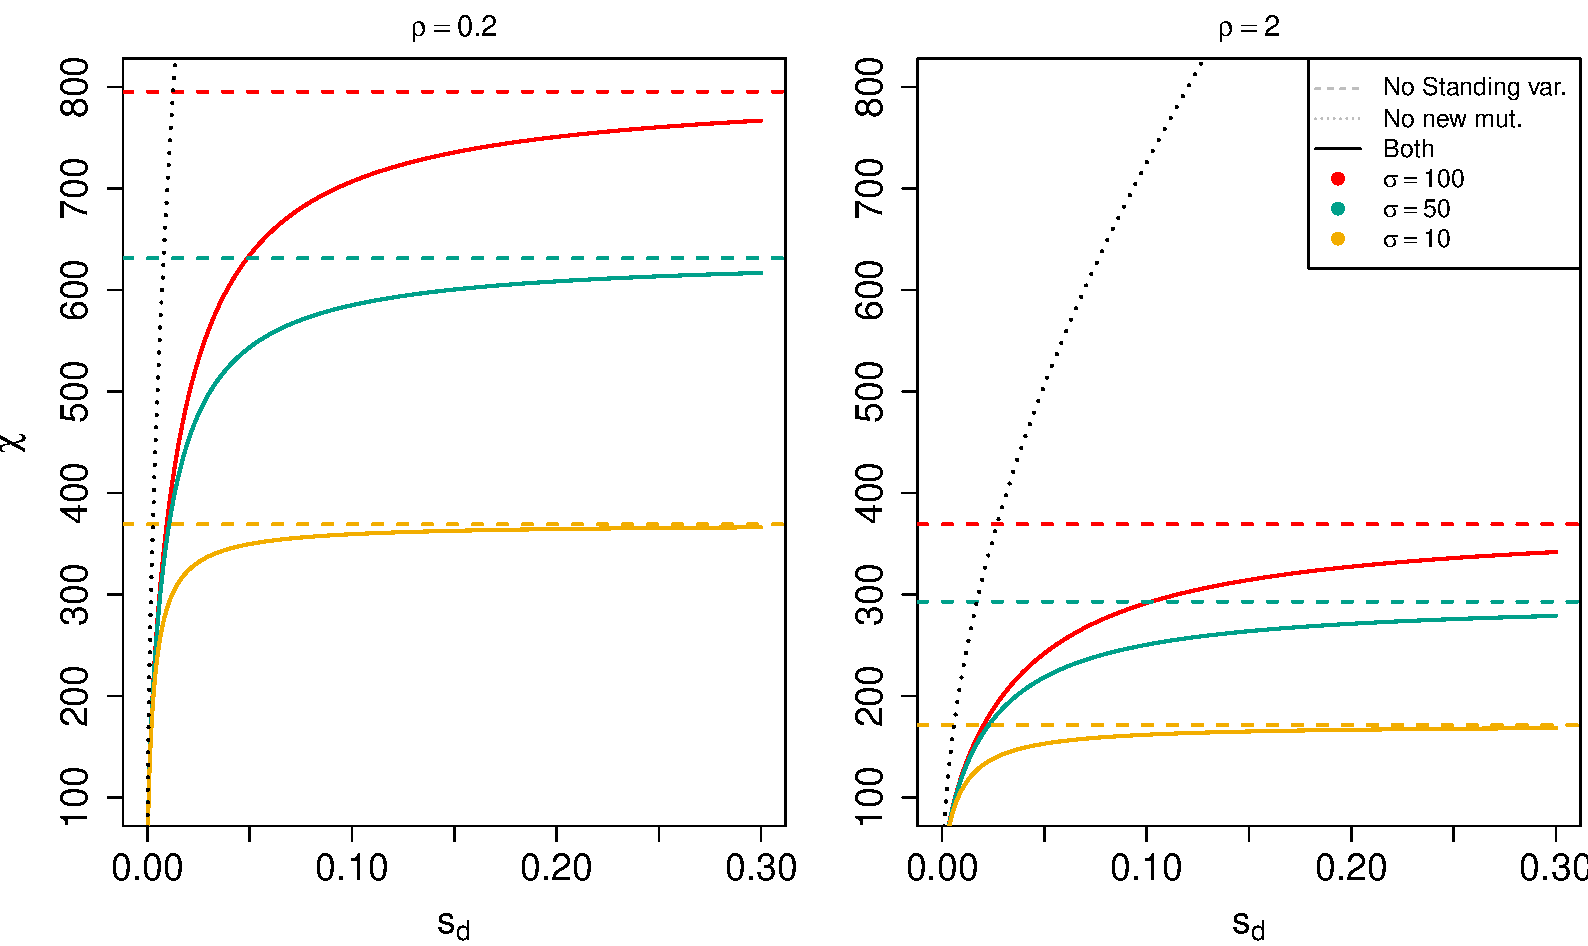
\includegraphics[width=1.0\textwidth]{G6PD_charlengths}   %{charlen-by-sd-limit}
\caption{ %
{\bf Characteristic length,} as a function of selective disadvantage, compared to the corresponding quantity without standing variation (e.g.\ from \cite{ralphcoop2010}) and to the quantity only considering standing variants (e.g.\ $\sqrt{\lambda_0}$).
} \label{Fig-G6PD-charlength}
\end{center}
\end{figure}

% \begin{figure}[ht]
% \begin{center}
%   \includegraphics[width=1.0\textwidth]{charlen-by-sd-sigma}
% \caption{ %
% {\bf Characteristic length,} as a function of dispersal distance $\sigma$ and selective disadvantage $s_d$.  XXX at what parameters. XXX
% }
% \end{center}
% \end{figure}


\subsection{Standing Variation -- Results} 

The quantity that is perhaps easiest to compute is the mean time until adaptation.
Fix some geographic location, and let $\tau\ge0$ be the time at which the point is reached by the advantageous mutations.
Then, as shown in Figure XX,
$\tau > t$ if and only if the cone with point at $(x,t)$ and slope $v$ extending back to $t=0$ is empty of successful mutations.
Since we assume these are a Poisson process, 
\[
    \P\{ \tau > t \} = \exp\left( - \lambda_0 \pi v^2 t^2 - \lambda \pi v^2 t^3 / 3 \right) ,
\]
and so we have
\begin{align}
    \E[\tau] % &= \int_0^\infty \P\{ \tau > t \} dt \\
        &= \int_0^\infty \exp\left( - \lambda_0 \pi v^2 t^2 - \lambda \pi v^2 t^3 / 3 \right) dt.
\end{align}
For means of evaluting this integral, see Appendix \ref{apx:integrals}.

In Figure \ref{G6PD_chartimes}

\begin{figure}[ht]
\begin{center}
  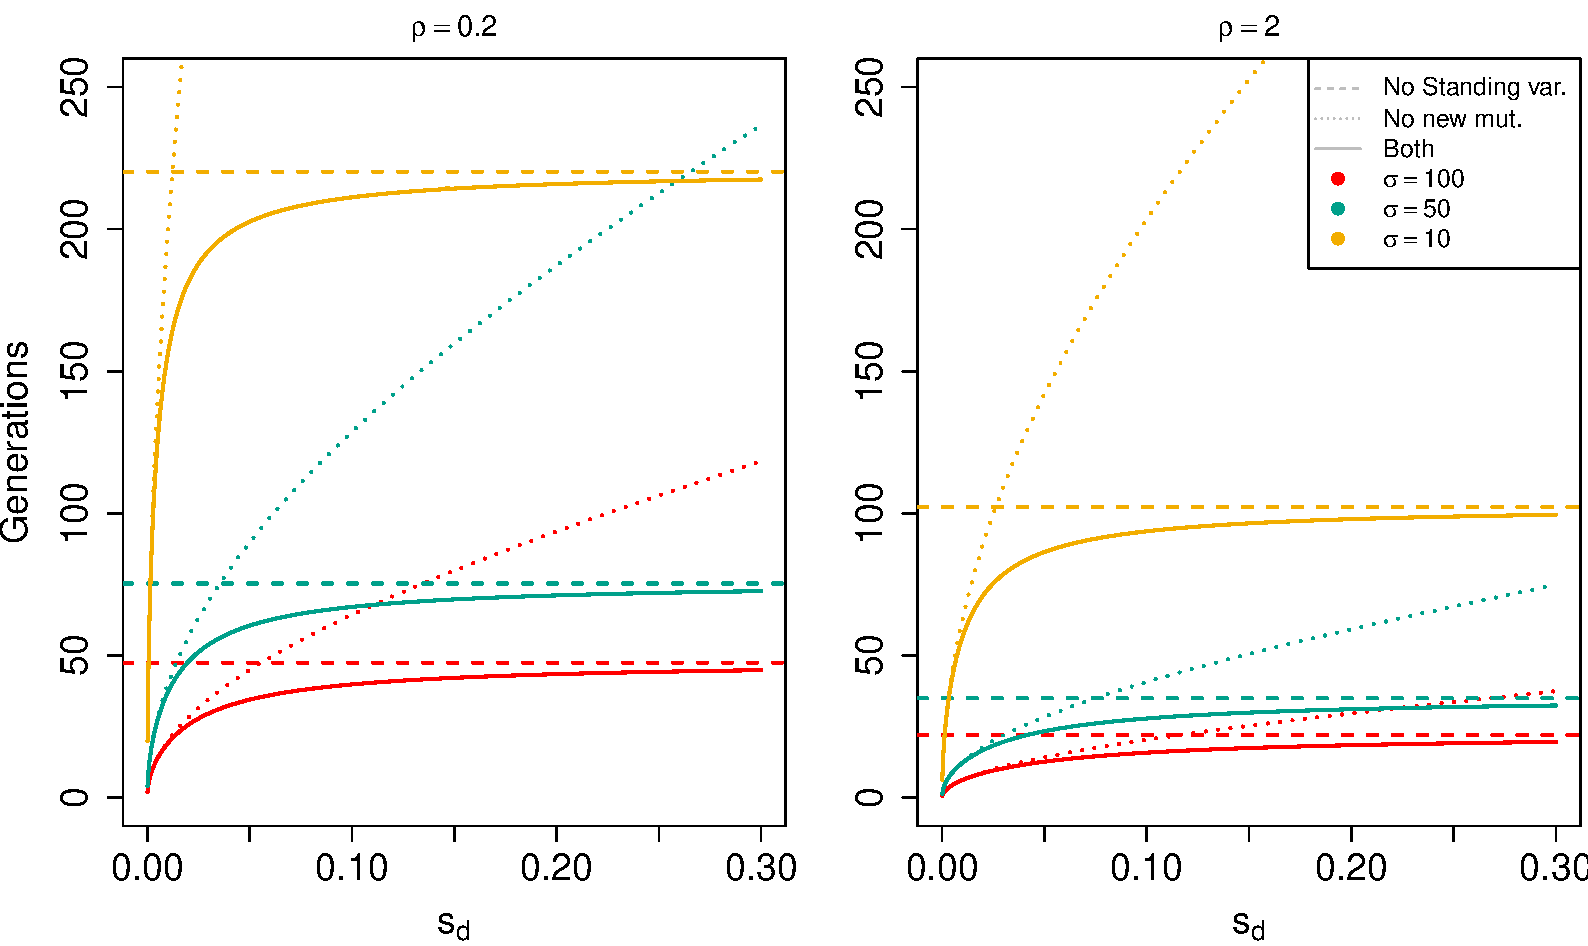
\includegraphics[width=1.0\textwidth]{G6PD_chartimes}   %{charlen-by-sd-limit}
\caption{ %
{\bf Mean adaptation times,} as a function of selective disadvantage, compared to the corresponding quantity without standing variation (e.g.\ from \cite{ralphcoop2010}) and to the quantity only considering standing variants (e.g.\ $\sqrt{\lambda_0}$).
} \label{G6PD_chartimes}
\end{center}
\end{figure}

% proportion of haplotypes (and of space) that are from standing variation 

We have defined $\lambda_0$ to be the mean density of standing variants that reach local fixation.
Define $\nu_+$ to be the mean density of new mutants whose offspring fix locally.
Since the probability that a mutant arising at $(x,t)$ is lucky enough to be born in a location not already occupied by mutants
is $\P\{ \tau > t \}$,
we can see  $\nu_+ = \int_0^\infty \lambda \P\{\tau>t\} dt$, and hence
$\nu_+ = \lambda \E[\tau] $.
Using that $\lambda_0 = \lambda / \log(1/(1-s_d))$, this gives us that
\begin{equation}
    \nu_+ = (\mbox{mean density of new patches}) = \frac{1}{1-\log(1-s_d) \E[\tau]} .
\end{equation}
Since the mean proportion of patches that come from standing variation is $\lambda_0 / (\lambda_0 + \nu_+)$,
this gives us the exact quantity we approximated by $\pi_0$ in \eqref{eqn:pizero}.
There are $\lambda_0 + \nu_+$ patches per unit area, so
the typical patch (i.e.\ with distribution given by the Palm measure) occupies area $1/(\lambda_0 + \nu_+)$.

We can also find the mean proportion of space covered by standing variants.
If by time $t$ a geographic location has not yet been reached by the mutation,
the probability it will be reached by time $t+dt$ 
by a standing variant is approximately $2 \lambda_0 \pi v^2 t dt$, 
and the probability it is reached by a new variant is $\lambda \pi v^2 t^2 dt$.
Therefore, as is standard for competing exponentials,
the probability a given location is reached first by a standing variant,
and therefore the mean proportion of space covered  by standing variants,
is
\begin{equation}
    z_0 = \int_0^\infty {2 \lambda_0 \pi v^2 t} \; \exp \left( - \lambda_0 \pi v^2 t^2 - \lambda \pi v^2 t^3 / 3 \right) dt .
\end{equation}
\marginnote{put in this value in terms of Gaussian CDF?}
To evaluate this integral, again see Appendix \ref{apx:integrals}.

Furthermore, if we define $a_0$ to be the mean area occupied by a typical standing variant, 
then $a_0$ is given by the proportion of the range occupied by standing variants over the mean density of unique standing variants,
i.e.\ $a_0 = z_0 / \lambda_0$.
We can compare this to the corresponding quantity $a_+$ for a new variant through the formula
$a_0 / a_+ = z_0 / (1-z_0)$.

In Figure \ref{G6PD_standing_var_proportion} 

\begin{figure}[ht]
\begin{center}
  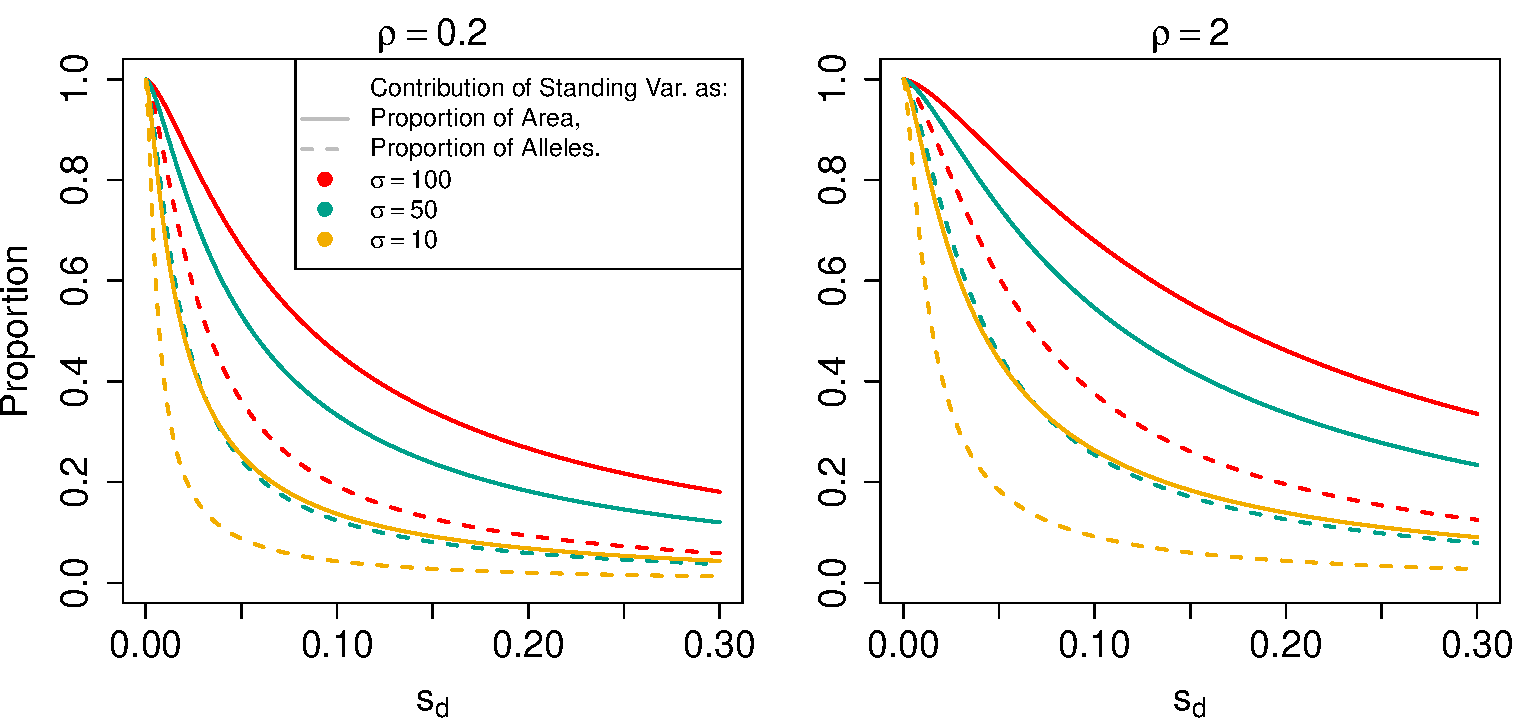
\includegraphics[width=1.0\textwidth]{G6PD_standing_var_proportion}
\caption{ %
{\bf Mean proportion of patches arising from standing variation.} The parameters given are for the sickle-cell example.  XXX say more.
} \label{G6PD_standing_var_proportion}
\end{center}
\end{figure}


\marginnote{do mean (and variance?) of distance between haplotypes?}

influence of migration on things -- plot these versus migration 

{\tt Simulations:} compare mean density against $s_d$ at different values of $\sigma$; omit variability if needed for readability.
Compare to panmictic results.


\subsubsection{Multiple variant types}

One interesting problem that we can seek to address with this work is
the extent to which 

Lets imagine for the moment that all classes of beneficial allele have
the same beneficial selection coefficient. 
Each class of mutations could have its own mutation rate $\mu_j$ and
have a disadvantage $s_{d,j}$ prior to the switch. As they have the
same selection coefficient all of the waves travel outward at a rate
$v$. 

\begin{align}
    \lambda_{0,j} = \frac{ 2 \mu_j \rho s_b }{ -\log(1-s_{d,j}) } ; ~~      \lambda_{j} = \mu_j \rho s_b;
\end{align}

\begin{equation}
    z_0 = \int_0^\infty {\lambda_{0,j} \pi v^2 t^2 - \lambda_j \pi v^2 t^3 / 3} \; \exp \left( - \lambda_{0,j} \pi v^2 t^2 - \lambda_j \pi v^2 t^3 / 3 \right) dt .
\end{equation}


\section{Local establishment and comparison to panmixia}

In the above (and in \citet{ralphcoop2010}) we have assumed that once the mutation appears,
conditional on eventual fixation, it begins to spread spatially at speed $v$ instantly,
effectively neglecting the time it must first spend fixing locally.
In \citet{ralphcoop2010} we addressed this by noting that there would be no change at all in our results 
if all mutations had to wait the same amount of time before fixing locally,
and that this time was short relative to the time it took the wave to spread across the characteristic length;
we then showed via simulation that this was reasonable in certain situations.
In this section we examine this assumption in more detail, although mostly through heuristic arguments,
and also compare our results above to those of \citet{softsweeps}.

We are assuming that shortly after a new mutation appears, 
it can be approximated by a branching process growing at rate $s$
until the point that it grows large enough to ``feel'' spatial structure,
at which point it begins to spread as a more--or--less deterministic wave.
Although we are not aware of good analysis of this transition, 
the relevant size when spatial structure becomes important
should be something close to $\sigma^2 \rho$ 
(i.e.\ Wright's ``local effective population size'' \citep{XXX}).
Let $Z_t$ be a continuous-time branching process with $Z_0=1$ and $\E[Z_t] = e^{s_b t}$.
Then we know that there exists a random variable $W$ such that $\lim_{t\to\infty} e^{-s_b t} Z_t = W$ almost surely,
so that if $\tau$ is the time $Z_t$ reaches size $\sigma^2 \rho$, i.e.\ $\tau = \inf\{ t \ge 0: Z_t > \sigma^2 \rho$,
then $\sigma^2 \rho = Z_\tau \approx e^{s_b \tau} W$.
From this we know that $\tau \approx (1/s_b) (\log (\sigma^2 \rho) - \log W)$;
although more detailed information is available (e.g.\ a CLT for $\tau$, \citet{XXX}),
we will stick to the loose interpretation.
\marginnote{check jaegers.  isn't there a CLT for $\tau$?}
As $\sigma^2 \rho$ increases, the mean of $\tau$ increases, but the variance approaches a constant
($\var[\tau] \to (1/s_b) \var[\log W]$).

So, roughly speaking, we need to evaluate the importance of a delay of about $T = (1/s_b) \log (\sigma^2 \rho)$.
New mutations will appear and fix during this time if $4N\mu s_b \ge 1/T$,
i.e.\ if $4 N \mu \ge 1/\log (\sigma^2 \rho)$.
Our model will still be a good approximation, however, 
as long as $T$ is short relative to the time a wave takes to spread between nearby mutational origins.
This can be worked out,
but it is simpler to note that if the converse is true, 
that the process is largely unaffected by spatial structure,
and so the panmictic model is a good approximation for the true process.
Since both our spatial model and the panmictic model underestimate the true degree of parallel adaptation,
it suffices to compare results from the two models to avoid applying the wrong model.

% When would we expect more mutations in this time?
% Roughly, if populations are larger than $C/\mu$ for some $C \approx 100$.
% Compare to panmixia: increases degree of parallel mutation if... ?

\citet{softsweepsII}, it is shown that under a panmictic model with certain assumptions on the parameters,
the number of independent origins due to both standing variation and new mutation seen in a sample of size $n$
has approximately the Ewens distribution with parameters $n$ and $\theta = 4 N \mu$.
As $n$ increases, the total number of types seen grows as $\log n$, 
so the ``mean density of types'' corresponding to our $\lambda_0 + \nu_+$ in their model is infinite.
\marginnote{Graph: sigma against mean number of origins; different curves for spatial, panmictic (flat), and simulation;
different values of theta as different line types?  but how to do this?
Mention Monty's empirical speeds paper.}
We could compare the probability of parallel adaptation under the two models (see eq'n 18 in \citet{softsweepsII}),
but this seems less useful than an assessment of the degree of parallel adaptation.


% \section{Applications}

% The FRIGIDA (FRI) in {\it  Arabidopsis thaliana} is a major
% determinant of genetic variation in flowering time. Recessive loss of function
% alleles at FRI result in early flowering, due to the almost complete
% loss the of the requirement of vernalization (a prolonged chill).  
% This is thought to potentially confer an advantage due to allowing a
% more rapid cycling life history. 

% Sweeps of FRI loss of function alleles \citep{Hagenblad-FRIsweep,Toomajian-FRIsweep}


% 20 independent nonfunctional FRI haplotypes \citep{Shindo-FRI}


% open reading frame (ORF) of 609 amino acids

\section{Discussion}

Thoughts
species coherence.
The Biological Reality of Species: Gene Flow, Selection, and Collective Evolution


\bibliography{standing_patches_refs}

\appendix

%%%%%%%%%%%%
\section{Integrals appearing in the text}
    \label{apx:integrals}

In the text at several points appear integrals of the form
\begin{align}
  \int_0^\infty t^c \exp \left( - \alpha t^d - \beta t^{d+1} \right) dt 
\end{align}
where $c$ is a positive integer, $d$ is the dimension, and $\alpha$ and $\beta$ are positive real numbers.
This could be evaluated through standard numerical methods; below we describe a power series expansion.
Changing variables to $u = \beta t^{d+1}$, this becomes
\begin{align}
    \left( (d+1)^{-1} \beta^{ (1-c)/(d+1) } \right) \int_0^\infty u^{(c+1-d)/(d+1)} \exp\left( - \alpha \beta^{-d/(d+1)} u^{d/(d+1)} - u \right) du ,
\end{align}
so it suffices to evaluate the function
\begin{equation}
    G(a,b,x) := \int_0^\infty  t^a \exp\left( -x t^b - t \right) dt ,
\end{equation}
in the case that $a=(c-d+1)/(d+1)$, $b=d/(d+1)$, and $x$ is a function of the demographic paramters.
Since $a$ and $b$ only depend on the dimension and the quantity being computed,
we are interested in $G$ as a function of $x$.
At least in the case $b=d/(d+1)$ it is possible to express $G$ as a finite sum of gamma functions,
but we proceed with a simpler method.
Note that $\partial_x G(a,b,x) = -G(a+b,b,x)$,
and that at $x=0$, the function $G$ is the gamma function $G(a,b,0) = \Gamma(a+1)$.
Therefore, a Taylor series for $G$ would be
\[
    G(a,b,x) = \sum_{n \ge 0} \frac{(-x)^n}{n!} \Gamma(a+nb+1) .
\]
It is easy to check using Stirling's formula that $\limsup_{n \to \infty} ( x^n \Gamma(a+nb+1)/n! )^{1/n} = 0$
if $b<1$, so the sum converges.


\end{document} 
